\documentclass[12pt]{article}

\usepackage{tikz}
\usetikzlibrary{positioning,arrows}

\begin{document}
	
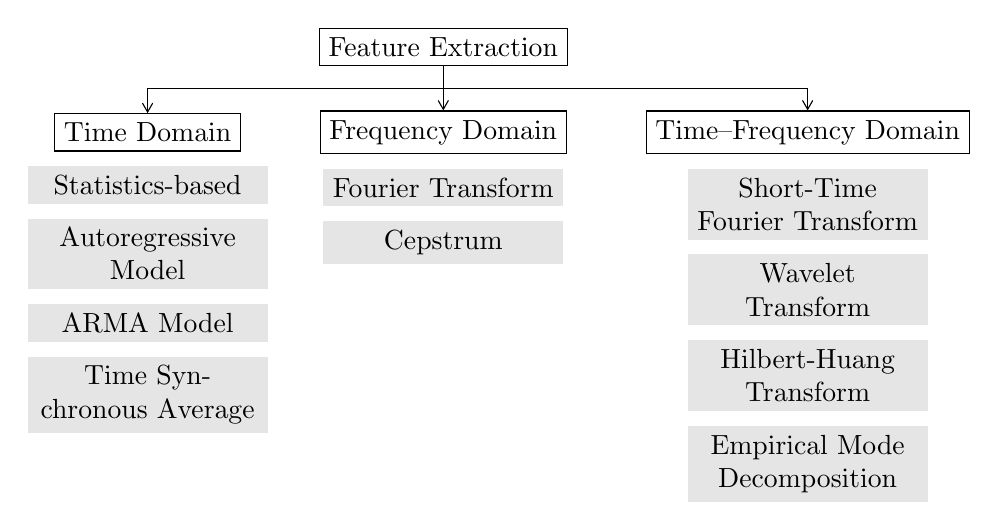
\begin{tikzpicture}
\tikzstyle{element}=[draw,rectangle]
\tikzstyle{entity}=[fill=gray!20,align=center, text width=8em]
\node[element] (fe) {Feature Extraction};


\node[element,below = 1.6em of fe] (fd) {Frequency Domain};
\node[element,left = of fd] (td) {Time Domain};
\node[element,right = of fd] (tfd) {Time--Frequency Domain};

\node[entity,below =.5em of td] (stat) {Statistics-based};
\node[entity,below =.5em of stat] (arm) {Autoregressive Model};
\node[entity,below =.5em of arm] (arma) {ARMA Model};
\node[entity,below =.5em of arma] (tsa) {Time Synchronous Average};

\node[entity,below =.5em of fd] (fft) {Fourier Transform};
\node[entity,below =.5em of fft] (cep) {Cepstrum};

\node[entity,below =.5em of tfd] (stft) {Short-Time Fourier Transform};
\node[entity,below =.5em of stft] (wt) {Wavelet Transform};
\node[entity,below =.5em of wt] (hht) {Hilbert-Huang Transform};
\node[entity,below =.5em of hht,align=center, text width=8em] (emd) {Empirical Mode Decomposition};

\draw[->,>=angle 60] (fe.south) -- ++(0,0) -- ++(0,-.8em) -| (td);
\draw[->,>=angle 60] (fe.south) -| (fd);
\draw[->,>=angle 60] (fe.south) -- ++(0,0) -- ++(0,-.8em) -| (tfd);
\end{tikzpicture}


\end{document}